\documentclass[12pt,a4paper]{article}

\input{preambulo.tex}
\input{portada.tex}

\usepackage{booktabs}
\usepackage{multirow}
\usepackage{listings}
\usepackage{xcolor}
\usepackage{subcaption}
\usepackage{array}
\usepackage{parskip}
\usepackage{titlesec}

% Definición de colores pastel y modernos
\definecolor{backcolour}{rgb}{0.96,0.96,0.96}
\definecolor{codegreen}{rgb}{0.13,0.55,0.13}
\definecolor{codegray}{rgb}{0.5,0.5,0.5}
\definecolor{codepurple}{rgb}{0.58,0,0.82}
\definecolor{codeblue}{rgb}{0.0,0.0,0.8}

% Definición de colores para gráficas
\definecolor{myblue}{RGB}{94, 52, 235}
\definecolor{myyellow}{RGB}{211, 121, 32}
\definecolor{myred}{RGB}{222, 75, 49}
\definecolor{mygreen}{RGB}{23, 110, 63}
        
% Configuración del estilo moderno
\lstdefinestyle{modern}{
    backgroundcolor=\color{backcolour},   
    commentstyle=\color{codegreen}\itshape,
    keywordstyle=\color{codeblue}\bfseries,
    numberstyle=\tiny\color{codegray},
    stringstyle=\color{codepurple},
    basicstyle=\ttfamily\scriptsize,
    breakatwhitespace=false,         
    breaklines=true,                 
    captionpos=b,                    
    keepspaces=true,                 
    numbers=left,                    
    numbersep=10pt,                  
    showspaces=false,                
    showstringspaces=false,
    showtabs=false,                  
    tabsize=4,
    frame=single,                    % Marco simple alrededor del código
    rulecolor=\color{lightgray},     % Color del marco
    xleftmargin=15pt,                % Margen para que los números no se peguen
    % --- Definición manual para tu Pseudocódigo ---
    morekeywords={Mientras, hacer, Para, hasta, Si, entonces, Si_no, Fin, Retornar, Inicializar, Evaluar, de},
    morecomment=[s]{(*}{*)},        % Define que (* *) es un comentario de bloque
    sensitive=false,                 % Hace que no distinga mayúsculas/minúsculas en las keywords
    % -----------------------------------------------------
    literate={á}{{\'a}}1 {é}{{\'e}}1 {í}{{\'i}}1 {ó}{{\'o}}1 {ú}{{\'u}}1
             {Á}{{\'A}}1 {É}{{\'E}}1 {Í}{{\'I}}1 {Ó}{{\'O}}1 {Ú}{{\'U}}1
             {ñ}{{\~n}}1 {Ñ}{{\~N}}1
}

% Aplicar el estilo por defecto a todos los bloques de código
\lstset{style=modern}

\begin{document}

\portada[%
        titulo=Metaheurísticas,
        subtitulo=Trabajo final:\\ Sine Cosine Algorithm (SCA),
        autor=Jesús Muñoz Velasco,
        año=Curso 2025-2026]
        
    \thispagestyle{empty}
    \tableofcontents
    \newpage
    \thispagestyle{empty}

% ----------------------------------------------------------------
\part{Descripción}

\section{Introducción y contexto}

El {Sine Cosine Algorithm} (SCA) es una metaheurística poblacional propuesta por Seyedali Mirjalili en 2016 en el artículo \textit{``SCA: A Sine Cosine Algorithm for solving optimization problems''} (Knowledge-Based Systems, vol.~96, pp.~120--133). Su propuesta se enmarca dentro de la familia de algoritmos basados en modelos matemáticos, también denominados \textit{math-inspired}, en contraposición a los inspirados en fenómenos biológicos o físicos.

El SCA parte de la idea de que las funciones seno y coseno poseen propiedades geométricas naturalmente útiles para la búsqueda: oscilan de forma periódica, pueden tomar valores superiores o inferiores al rango $[-1,1]$ si se escalan convenientemente, y su comportamiento alternante facilita tanto la exploración global del espacio de búsqueda como la explotación local alrededor de soluciones prometedoras. Desde su publicación, el algoritmo ha atraído una atención considerable en la comunidad investigadora, siendo aplicado en campos tan diversos como la ingeniería eléctrica, el aprendizaje automático, el diagnóstico médico y la planificación de rutas.

% ----------------------------------------------------------------
\section{Fundamentos matemáticos}
\subsection{Ecuaciones de actualización de posición}

Cada candidato a solución (denominado \textit{agente de búsqueda}) se representa como un vector $\mathbf{X}^t \in \mathbb{R}^d$, donde $d$ es la dimensión del problema y $t$ el instante de iteración. En cada paso, el agente actualiza su posición {dimensión a dimensión} según:

\begin{equation}
X_i^{t+1} =
\begin{cases}
X_i^t + r_1 \cdot \sin(r_2) \cdot \left| r_3 P_i^t - X_i^t \right|, & \text{si } r_4 < 0{,}5 \\[6pt]
X_i^t + r_1 \cdot \cos(r_2) \cdot \left| r_3 P_i^t - X_i^t \right|, & \text{si } r_4 \geq 0{,}5
\end{cases}
\label{eq:update}
\end{equation}

La ecuación puede factorizarse para visualizarla mejor. Definiendo el \textit{desplazamiento escalado} $\Delta_i^t = r_3 P_i^t - X_i^t$ (distancia ponderada al destino, con signo) y el \textit{factor trigonométrico} $\phi = r_1 \cdot f(r_2)$ donde $f \in \{\sin, \cos\}$, la actualización se reduce a:

\begin{equation}
X_i^{t+1} = X_i^t + \phi \cdot |\Delta_i^t|
\label{eq:factored}
\end{equation}

El valor absoluto $|\Delta_i^t|$ garantiza que la {magnitud} del paso sea siempre positiva; el {signo} del movimiento queda determinado enteramente por $\phi$: si $\phi > 0$ el agente avanza hacia el destino (o más allá), si $\phi < 0$ retrocede. Esta separación entre magnitud y dirección es lo que confiere al SCA su capacidad para cubrir simétricamente el espacio alrededor del punto destino.

Los cuatro parámetros tienen roles bien diferenciados:

\begin{center}
\begin{tabular}{c l l}
\toprule
\textbf{Param.} & \textbf{Rango} & \textbf{Rol en la actualización} \\
\midrule
$r_1$ & $[0,\,a]$ decreciente & Amplitud del movimiento (exploración/explotación) \\
$r_2$ & $[0,\,2\pi]$ aleatorio & Ángulo trigonométrico (dirección y signo del paso) \\
$r_3$ & $[0,\,2]$ aleatorio  & Peso estocástico de la distancia al destino \\
$r_4$ & $[0,\,1]$ aleatorio  & Selección equiprobable de seno o coseno \\
\bottomrule
\end{tabular}
\end{center}

\subsection{Papel de cada parámetro}

\subsubsection{El parámetro $r_1$: transición exploración/explotación}

$r_1$ es el parámetro de mayor importancia. Viene dado por\footnote{El parámetro $a$ se toma igual a 2 para que el espacio de búsqueda alrededor del punto destino quede completamente cubierto desde el principio (está acotado por el doble de la distancia inicial), además de que con este valor, el umbral $r_1=1$ se alcanza exactamente en $t=\nicefrac{T}{2}$ dividiendo las iteraciones perfectamente por la mitad para exploración y explotación. Aún así se puede tomar otro valor para darle más relevancia a alguna de estas fases.}

\begin{equation}
r_1(t) = a \left(1 - \frac{t}{T}\right), \qquad a = 2
\label{eq:r1}
\end{equation}

Como se puede ver comienza con el valor $a$ ($r_1(0)=a$) y va descendiendo linealmente hasta $0$ ($r_1(T)=0$) a lo largo de las iteraciones.

La Figura~\ref{fig:r1} muestra su trayectoria y el umbral $r_1 = 1$ que separa las dos regiones:

\begin{itemize}
  \item \textbf{Exploración} ($r_1 \geq 1$, primeras iteraciones): el factor $r_1 \cdot f(r_2)$ puede superar en módulo la distancia $|\Delta_i^t|$, de modo que el agente sobrepasa el punto destino y explora regiones lejanas del espacio.
  \item \textbf{Explotación} ($r_1 < 1$): el factor queda acotado y el agente se mueve dentro del segmento que lo une con el destino, refinando la solución progresivamente.
\end{itemize}

\begin{figure}[H]
\centering

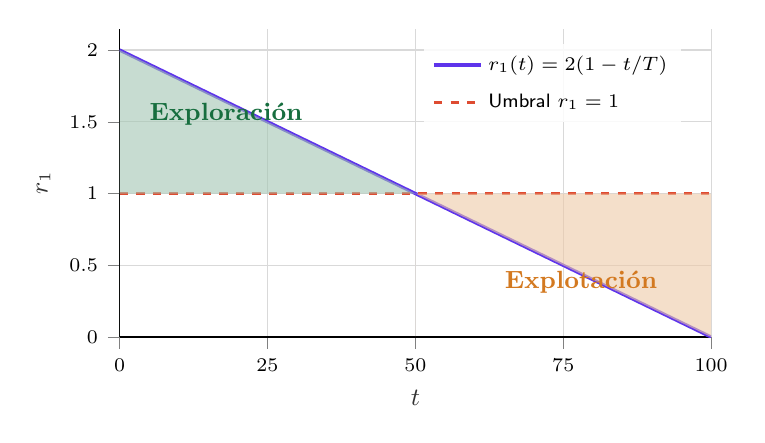
\begin{tikzpicture}
\begin{axis}[
  width=0.75\textwidth, height=5.5cm,
  % --- Estilo de Ejes Moderno ---
  axis lines*=left,                 % Elimina las líneas superior y derecha (gráfico abierto)
  axis line style={draw=black, line width=0.6pt},
  % --- Etiquetas y Texto ---
  xlabel={$t$},
  ylabel={$r_1$},
  label style={font=\small\sffamily, text=black!80},
  tick label style={font=\scriptsize\sffamily, text=black},
  % --- Límites y Ticks ---
  xmin=0, xmax=100,
  ymin=0, ymax=2.15,
  xtick={0,25,50,75,100},
  ytick={0,0.5,1,1.5,2},
  tick align=outside,               % Ticks hacia afuera para no obstruir los datos
  % --- Grilla Sutil ---
  grid=both,
  grid style={line width=0.4pt, draw=gray!30},
  % --- Leyenda Limpia ---
  legend style={
    font=\scriptsize\sffamily, 
    at={(0.95,0.95)}, 
    anchor=north east,
    draw=none,                      % Sin borde negro rígido
    fill=white, 
    fill opacity=0.85,              % Fondo ligeramente translúcido
    text opacity=1,
    row sep=3pt
  },
  legend cell align={left},         % Alinea el texto de la leyenda a la izquierda
]
  %% Línea r1 decreciente
  \addplot[very thick, myblue, domain=0:100, samples=200]
    {2*(1 - x/100)};
  \addlegendentry{$r_1(t) = 2(1-t/T)$}

  %% Umbral r1 = 1
  \addplot[very thick, dashed, myred, domain=0:100, samples=2]
    {1};
  \addlegendentry{Umbral $r_1 = 1$}

  %% Relleno zona exploración
  \addplot[fill=mygreen!40, opacity=0.6, draw=none]
    coordinates {(0,2)(50,1)(50,1)(0,1)} \closedcycle;

  %% Relleno zona explotación
  \addplot[fill=myyellow!40, opacity=0.6, draw=none]
    coordinates {(50,1)(100,0)(100,1)(50,1)} \closedcycle;

  %% Etiquetas de zona
  \node[font=\small\bfseries, mygreen]  at (axis cs:18, 1.55) {Exploración};
  \node[font=\small\bfseries, myyellow] at (axis cs:78, 0.38) {Explotación};

\end{axis}
\end{tikzpicture}
\caption{Evolución de $r_1$ a lo largo de las iteraciones ($a=2$, $T=100$). La región azul corresponde a la fase de exploración ($r_1\geq 1$) y la naranja a la de explotación ($r_1 < 1$). El cruce ocurre exactamente en $t = T/2$.}
\label{fig:r1}
\end{figure}


\subsubsection{El parámetro $r_2$: dirección del movimiento}

$r_2$ es el ángulo de la función trigonométrica, muestreado uniformemente en $[0, 2\pi]$. Su efecto se aprecia analizando el signo de $\sin(r_2)$ y $\cos(r_2)$:

\begin{itemize}
  \item Cuando $f(r_2) > 0$ el desplazamiento es positivo: el agente se mueve en la dirección de $P_i - X_i$ (hacia el destino o más allá).
  \item Cuando $f(r_2) < 0$ el desplazamiento es negativo: el agente se aleja del destino en esa dimensión.
\end{itemize}

La Figura~\ref{fig:trig} representa $r_1 \cdot \sin(r_2)$ y $r_1 \cdot \cos(r_2)$ para dos valores representativos de $r_1$, mostrando cómo la amplitud se contrae al pasar de la fase exploratoria a la explotadora.

\begin{figure}[H]
\centering
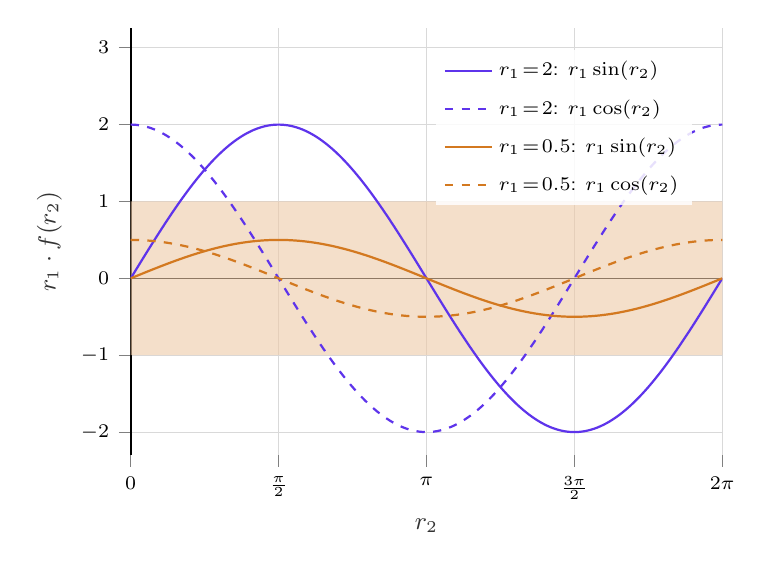
\begin{tikzpicture}
\begin{axis}[
  width=0.75\textwidth, height=7cm,
  % --- Estilo de Ejes Moderno ---
  axis lines*=left,                 % Elimina las líneas superior y derecha (gráfico abierto)
  x axis line style={draw=none},  % Eliminamos el eje X para ponerlo personalizado en y=0
  y axis line style={draw=black, line width=0.6pt},
  % --- Etiquetas y Texto ---
  xlabel={$r_2$},
  ylabel={$r_1 \cdot f(r_2)$},
  label style={font=\small\sffamily, text=black!80},
  tick label style={font=\scriptsize\sffamily, text=black},
  % --- Límites y Ticks ---
  xmin=0, xmax=6.2832,
  ymin=-2.3, ymax=3.25,
  xtick={0, 1.5708, 3.1416, 4.7124, 6.2832},
  xticklabels={$0$, $\frac{\pi}{2}$, $\pi$, $\frac{3\pi}{2}$, $2\pi$},
  ytick={-2,-1,0,1,2, 3},
  tick align=outside,               % Ticks hacia afuera para no obstruir los datos
  % --- Grilla Sutil ---
  grid=both,
  grid style={line width=0.4pt, draw=gray!30},
  % --- Leyenda Limpia ---
  legend style={
    font=\scriptsize\sffamily, 
    at={(0.95,0.95)}, 
    anchor=north east,
    draw=none,                      % Sin borde negro rígido
    fill=white, 
    fill opacity=0.85,              % Fondo ligeramente translúcido
    text opacity=1,
    row sep=3pt
  },
  legend cell align={left},         % Alinea el texto de la leyenda a la izquierda
]

    %% Eje X
    \addplot[draw=black, line width=0.6pt, domain=0:6.2832, forget plot]
    {0};

    %% Zona de explotación: |valor| <= 1
    \addplot[fill=myyellow!40, opacity=0.6, draw=none, domain=0:6.2832, samples=3, forget plot]
        coordinates {(0,-1)(6.2832,-1)(6.2832,1)(0,1)} \closedcycle;

    %% Zona de exploración: |valor| > 1
    % \addplot[fill=mygreen!40, opacity=0.6, draw=none, domain=0:6.2832, samples=3, forget plot]
    %     coordinates {(0,1)(6.2832,1)(6.2832,3.25)(0,3.25)} \closedcycle;
    % \addplot[fill=mygreen!40, opacity=0.6, draw=none, domain=0:6.2832, samples=3, forget plot]
    %     coordinates {(0,-1)(6.2832,-1)(6.2832,-2.3)(0,-2.3)} \closedcycle;

    %% r1=2 (exploración): seno
    \addplot[thick, myblue, domain=0:6.2832, samples=200]
        { 2*sin(deg(x)) };
    \addlegendentry{$r_1\!=\!2$: $r_1\sin(r_2)$}

    %% r1=2: coseno (discontinuo azul)
    \addplot[thick, myblue, dashed, domain=0:6.2832, samples=200]
        { 2*cos(deg(x)) };
    \addlegendentry{$r_1\!=\!2$: $r_1\cos(r_2)$}

    %% r1=0.5 (explotación): seno
    \addplot[thick, myyellow, domain=0:6.2832, samples=200]
        { 0.5*sin(deg(x)) };
    \addlegendentry{$r_1\!=\!0.5$: $r_1\sin(r_2)$}

    %% r1=0.5: coseno
    \addplot[thick, myyellow, dashed, domain=0:6.2832, samples=200]
        { 0.5*cos(deg(x)) };
    \addlegendentry{$r_1\!=\!0.5$: $r_1\cos(r_2)$}

\end{axis}
\end{tikzpicture}
\caption{Factor trigonométrico $r_1 \cdot f(r_2)$ en función del ángulo $r_2$ para $r_1=2$ (exploración, azul) y $r_1=0{,}5$ (explotación, naranja). La banda sombreada $[-1,1]$ delimita el régimen de explotación: cuando el factor queda dentro de ella, el agente no sobrepasa el destino.}
\label{fig:trig}
\end{figure}

\subsubsection{Los parámetros $r_3$ y $r_4$}

$r_3 \in [0, 2]$ actúa como un peso estocástico sobre el punto destino. Si $r_3 > 1$, el término $r_3 P_i^t$ desplaza el destino efectivo más allá de su posición real, ampliando artificialmente la distancia $|\Delta_i^t|$ y favoreciendo pasos más largos (efecto exploratorio secundario). Si $r_3 < 1$, atenúa la influencia del destino. Este mecanismo introduce diversidad adicional incluso en la fase de explotación, reduciendo el riesgo de convergencia en masa hacia un único punto.

$r_4 \in [0,1]$ selecciona con probabilidad $1/2$ entre la función seno y la función coseno. Ambas funciones tienen la misma amplitud máxima, pero sus ceros y máximos están desfasados $\pi/2$ radianes. Emplearlas con igual probabilidad garantiza que el muestreo de direcciones de movimiento sea más uniforme que si se usase una sola función, mejorando la isotropía de la búsqueda en el espacio.

\subsection{Geometría de la búsqueda}

La ecuación~\eqref{eq:factored} actualiza cada dimensión de forma independiente. En una dimensión fija $j$, el nuevo valor del agente es:
\[
  X_j^{t+1} = X_j^t + \phi \cdot |\Delta_j^t|,
  \qquad |\Delta_j^t| = |r_3 P_j^t - X_j^t|, \qquad \phi = r_1 \cdot f(r_2)
\]
donde $|\Delta_j^t| \geq 0$ siempre. Por tanto, el signo y la magnitud del desplazamiento quedan determinados exclusivamente por $\phi$, que puede tomar cualquier valor real en $[-r_1,\, r_1]$. Esto da lugar a cuatro regímenes de movimiento, representados en la Figura~\ref{fig:geometry}:

\begin{itemize}
  \item $\phi \in (0,1)$: explotación positiva. El agente se desplaza hacia $P_j^t$ sin alcanzarlo.
  \item $\phi \in (-1,0)$: explotación negativa. El agente retrocede levemente desde $P_j^t$, pero permanece cerca.
  \item $\phi > 1$: exploración positiva. El agente sobrepasa $P_j^t$ y aterriza más allá.
  \item $\phi < -1$: exploración negativa. El agente da un salto largo en sentido opuesto a $P_j^t$.
\end{itemize}

Como ya se ha comentado, los casos $|\phi| < 1$ constituyen la zona de explotación y los casos $|\phi| > 1$ la zona de exploración. El umbral es exactamente $|\phi| = 1$, que corresponde al punto $P_j^t$ escalado por $r_3$. Nótese que las zonas de exploración son simétricas a ambos lados del agente, lo que garantiza que la búsqueda no tenga sesgo de dirección.

\begin{figure}[H]
\centering
\begin{tikzpicture}[>=Stealth, thick, font=\small]

  %% --- Coordenadas clave ---
  \coordinate (X) at (0,0);
  \coordinate (P) at (4,0);

  %% --- Bandas de fondo (primero, para que queden detrás) ---
  % Explotación: entre -|Delta| y +|Delta| alrededor de X
  \fill[myyellow!40, opacity=0.6] (-4,-0.35) rectangle (4, 0.35);
  % Exploración positiva (más allá de P)
  \fill[mygreen!40, opacity=0.6]   ( 4,-0.35) rectangle (7, 0.35);
  % Exploración negativa (más allá de -P)
  \fill[mygreen!40, opacity=0.6]   (-4,-0.35) rectangle (-7,0.35);

  %% --- Eje horizontal ---
  \draw[gray!50, thin] (-6.8,0) -- (6.8,0);

  %% --- Cota de distancia |Delta| ---
  \draw[<->, gray!60, thin] (0,-0.75) -- (4,-0.75)
      node[midway, below, gray!80] {\footnotesize $|\Delta_j^t|$};
  \draw[dashed, gray!50, thin] (4, 0) -- (4,-0.9);
  \draw[dashed, gray!50, thin] (0,0) -- (0,-0.9);
  

  %% --- Cuatro flechas de movimiento ---

  % (3) Exploración positiva: phi > 1
  \draw[->, thick, myblue] (0,0) -- (5.8, 0)
      node[above] {\footnotesize $\phi\!>\!1$};

  % (4) Exploración negativa: phi < -1
  \draw[->, thick, teal!70!black] (0,0) -- (-5.5,-0)
      node[above] {\footnotesize $\phi\!<\!-1$};

  % (1) Explotación positiva: phi in (0,1)
  \draw[->, very thick, myyellow!80!black] (0,0) -- (2.5, 0)
      node[below] {\footnotesize $0 \!<\!\phi\!<1$};

  % (2) Explotación negativa: phi in (-1,0)
  \draw[->, very thick, myyellow] (0,0) -- (-2.0,0)
      node[below] {\footnotesize $-1 \!<\!\phi\!<0$};

  %% --- Etiquetas de zona ---
  \node[myyellow, font=\footnotesize\bfseries] at ( 0,  1.1)
      {Explotación};
  \node[mygreen, font=\footnotesize\bfseries] at ( 5.5, 1.1)
      {Exploración};
  \node[mygreen, font=\footnotesize\bfseries] at (-5.5, 1.1)
      {Exploración};

  %% --- Puntos ---
  \filldraw[myred]          (P) circle (3pt);

  \node[above=4pt, myred]   at (P)  {$P_j^t$};

  \filldraw[black]         (X) circle (3pt);
  \node[above=4pt, black]  at (X) {$X_j^t$};

\end{tikzpicture}
\caption{Cuatro regímenes de movimiento en una dimensión $j$. La banda amarilla ($|\phi|<1$) es la zona de {explotación}: el agente aterriza entre $X_j^t$ y el destino (o su simétrico). Las bandas azul y verde ($|\phi|>1$) son zonas de {exploración}: el agente sobrepasa el destino en alguno de los dos sentidos. La simetría horizontal garantiza la ausencia de sesgo direccional.}
\label{fig:geometry}
\end{figure}

Desde una perspectiva probabilística, el valor esperado de $|\phi|$ decrece con $t$ al hacerlo $r_1$, ya que
\begin{equation*}
    E[|\phi|] = r_1 \cdot E[|f(r_2)|] = r_1 \cdot \frac{2}{\pi}
\end{equation*}
Esto convierte la dinámica colectiva en un proceso de enfriamiento implícito: al inicio los agentes realizan saltos amplios y divergentes conforme avanza la búsqueda los pasos se acortan y la población converge hacia el punto destino con precisión creciente. El factor $2/\pi \approx 0{,}637$ implica además que, en promedio, el umbral efectivo de exploración/explotación se alcanza antes de que $r_1$ llegue a $1$, lo que supone una transición algo más temprana de lo que la ecuación~\eqref{eq:r1} sugiere a simple vista.

% ----------------------------------------------------------------
\section{Descripción del algoritmo}

\subsection{Pseudocódigo}

\begin{lstlisting}[caption={Pseudocódigo del Sine Cosine Algorithm (SCA)}, label={lst:sca}]
(* Parámetros de entrada: N (población), T (iteraciones máx.), a=2 *)
Inicializar población X = {X_1, X_2, ..., X_N} aleatoriamente en [lb, ub]^d
Evaluar fitness f(X_i) para cada agente i
P <- argmin f(X_i)    (* mejor solución: punto destino *)

t <- 1
Mientras t <= T hacer
    (* Calcular parámetro adaptativo r1 *)
    r1 <- a - t * (a / T)

    Para cada agente i = 1 hasta N hacer
        Para cada dimensión j = 1 hasta d hacer
            (* Generar parámetros aleatorios *)
            r2 <- aleatorio en [0, 2*pi]
            r3 <- aleatorio en [0, 2]
            r4 <- aleatorio en [0, 1]

            (* Actualizar posición según Ec. (1) *)
            Si r4 < 0.5 entonces
                X_i[j] <- X_i[j] + r1 * sin(r2) * |r3*P[j] - X_i[j]|
            Si_no
                X_i[j] <- X_i[j] + r1 * cos(r2) * |r3*P[j] - X_i[j]|
            Fin Si

            (* Aplicar límites del espacio de búsqueda *)
            X_i[j] <- max(lb[j], min(ub[j], X_i[j]))
        Fin Para
    Fin Para

    (* Evaluar fitness y actualizar punto destino *)
    Para cada agente i = 1 hasta N hacer
        Evaluar f(X_i)
        Si f(X_i) < f(P) entonces
            P <- X_i
        Fin Si
    Fin Para

    t <- t + 1
Fin Mientras

Retornar P   (* mejor solución encontrada *)
\end{lstlisting}

\subsection{Complejidad computacional}

La complejidad por iteración es $\mathcal{O}(N \cdot d)$, equivalente a la de otros algoritmos poblacionales estándar como PSO o GWO. El número total de evaluaciones de la función objetivo es $N \times T$, lo que resulta razonable para problemas de mediana escala.

% ----------------------------------------------------------------
\section{Por qué funciona el SCA}

El éxito del SCA descansa en tres pilares fundamentales:

\textbf{1. Balance exploración--explotación adaptativo.}  La reducción lineal de $r_1$ de $a$ a $0$ a lo largo de las iteraciones crea de forma natural una transición suave de la fase exploratoria (valores grandes de $r_1$ permiten saltos amplios) a la explotadora (valores pequeños de $r_1$ confinan el movimiento). Este mecanismo automático evita que el diseñador tenga que ajustar empíricamente la transición entre fases.

\textbf{2. Diversidad mediante aleatoriedad estructurada.}  Los parámetros $r_2$, $r_3$ y $r_4$ introducen aleatoriedad en la dirección, magnitud y función trigonométrica empleada, respectivamente. Esta triple fuente de variabilidad mantiene la diversidad de la población durante la búsqueda y reduce la probabilidad de convergencia prematura.

\textbf{3. Oscilación periódica como mecanismo de escape.}  Las propiedades oscilantes del seno y el coseno permiten que los agentes alteren su dirección de movimiento de manera natural. En particular, en las iteraciones iniciales los valores fuera del rango $[-1,1]$ actúan como operadores de perturbación implícitos, similares a las mutaciones en los algoritmos evolutivos, facilitando la salida de óptimos locales.

% ----------------------------------------------------------------
\section{Ventajas e inconvenientes}

\begin{table}[h!]
\centering
\renewcommand{\arraystretch}{1.35}
\begin{tabular}{>{\bfseries}p{0.44\textwidth} p{0.44\textwidth}}
\toprule
Ventajas & Inconvenientes \\
\midrule
Implementación simple: pocos parámetros ($a$, $N$, $T$).
&
Tendencia a la convergencia prematura en funciones multimodales complejas de alta dimensión.
\\
Buen equilibrio exploración/explotación gracias al decaimiento de $r_1$.
&
La actualización lineal de $r_1$ no se adapta a la forma del paisaje de aptitud; puede ser subóptima en problemas no lineales.
\\
Convergencia competitiva frente a PSO, GA y GWO en benchmarks estándar.
&
Baja diversidad en iteraciones avanzadas, lo que favorece el estancamiento en óptimos locales.
\\
Bajo costo computacional por iteración: $\mathcal{O}(N \cdot d)$.
&
Escasa memoria colectiva: los agentes no comparten información entre ellos más allá del punto destino global.
\\
Flexibilidad: fácilmente hibridable con otros algoritmos (PSO, DE, ABC).
&
Rendimiento degradado en espacios de búsqueda discretos o combinatorios sin adaptaciones adicionales.
\\
\bottomrule
\end{tabular}
\caption{Resumen de ventajas e inconvenientes del SCA.}
\label{tab:pros_cons}
\end{table}

% ----------------------------------------------------------------
\section{Cuándo funciona bien}

El SCA muestra su mejor rendimiento en los siguientes contextos:

\begin{itemize}
  \item \textbf{Problemas continuos de dimensión baja o media} ($d \leq 100$): la oscilación controlada por $r_1$ es suficiente para cubrir el espacio de búsqueda sin necesidad de operadores adicionales.
  \item \textbf{Funciones unimodales o con pocos óptimos locales}: la convergencia progresiva resulta adecuada cuando el paisaje de aptitud no presenta muchas trampas locales.
  \item \textbf{Situaciones con restricciones presupuestarias de evaluación}: su bajo overhead computacional lo hace conveniente cuando la evaluación de la función objetivo es costosa y el número de iteraciones debe minimizarse.
  \item \textbf{Problemas de ingeniería clásicos con restricciones}: diseño de estructuras, optimización de parámetros de máquinas, flujo de potencia óptimo, donde la superficie de aptitud es relativamente suave.
\end{itemize}

Por el contrario, el SCA original tiene dificultades en problemas combinatorios puros, funciones con numerosos óptimos locales (CEC2017 con alta dimensionalidad) o cuando se requiere una precisión de convergencia muy elevada.

% ----------------------------------------------------------------
\section{Aplicaciones en casos reales}

Desde 2016, el SCA ha sido adaptado y aplicado en una amplia variedad de dominios:

\textbf{Sistemas de potencia y energía.} El SCA ha sido empleado para resolver el problema de \textit{Optimal Power Flow} (OPF), minimizando pérdidas en redes eléctricas y optimizando la ubicación de compensadores estáticos de VAR (D-STATCOM) en sistemas de distribución. También se ha aplicado en la calendarización hidrotérmica a corto plazo.

\textbf{Selección de características y aprendizaje automático.} Se han propuesto versiones binarias del SCA (mediante funciones de transferencia en S o V) para selección de características en conjuntos de datos médicos, con resultados competitivos en precisión de clasificación. Asimismo, se ha utilizado para optimizar los hiperparámetros de máquinas de soporte vectorial (SVR) y redes neuronales multicapa.

\textbf{Segmentación de imágenes y diagnóstico médico.} El SCA se ha aplicado a la segmentación de imágenes médicas (resonancia magnética, tomografía computarizada) mediante el enfoque de umbrali\-zación multinivel. También ha sido empleado en el diagnóstico de cáncer de pulmón y en el ajuste de parámetros de modelos fotovoltaicos.

\textbf{Ingeniería mecánica y estructural.} Entre las aplicaciones destacan el diseño óptimo de la sección transversal de perfiles aerodinámicos, la optimización de sistemas de engranajes, la detección de daños estructurales y el diseño de componentes de automóviles.

\textbf{Robótica y telecomunicaciones.} El SCA ha sido utilizado para la planificación de trayectorias de robots (incluyendo vehículos autónomos subacuáticos) y para la colocación óptima de cámaras en sistemas de vigilancia y redes de sensores inalámbricos.

% ----------------------------------------------------------------
\section{Variantes y extensiones}

La comunidad ha propuesto numerosas mejoras al SCA original para paliar sus limitaciones:

\begin{itemize}
  \item \textbf{SCA-PSO / ASCA-PSO}: hibridación con Particle Swarm Optimization para mejorar la explotación local.
  \item \textbf{OBSCA}: incorpora aprendizaje por oposición (\textit{opposition-based learning}) para aumentar la diversidad inicial.
  \item \textbf{SCA caótico}: sustituye los parámetros aleatorios por mapas caóticos (logístico, de Chebyshev) para mejorar la cobertura del espacio.
  \item \textbf{MO-SCA}: extensión multi-objetivo que mantiene un archivo de soluciones Pareto-óptimas.
  \item \textbf{SCA binario}: adapta la actualización continua al espacio $\{0,1\}^d$ para problemas de selección de características.
  \item \textbf{EBSCA}: refuerza la fase de explotación mediante una ecuación de actualización centrada en el mejor individuo con un factor de equilibrio dinámico.
\end{itemize}

% ----------------------------------------------------------------
\section{Conclusiones}

El Sine Cosine Algorithm es una metaheurística elegante, de implementación sencilla y costo computacional reducido, que aprovecha las propiedades oscilantes y periódicas de las funciones trigonométricas para navegar el espacio de búsqueda. Su mecanismo de transición automática entre exploración y explotación, basado en el decaimiento lineal de $r_1$, lo convierte en un punto de partida eficaz para una amplia gama de problemas continuos de optimización. Sin embargo, como dicta el teorema \textit{No Free Lunch}, el SCA no es universalmente superior: en problemas altamente multimodales o de gran dimensión su convergencia puede estancarse en óptimos locales y su limitada memoria colectiva reduce la calidad de las soluciones. La rica familia de variantes híbridas y mejoradas surgidas desde 2016 refleja tanto el interés de la comunidad como el espacio de mejora existente sobre la versión original.

% ----------------------------------------------------------------
\begin{thebibliography}{9}

\bibitem{mirjalili2016}
S.~Mirjalili,
\textit{SCA: A Sine Cosine Algorithm for solving optimization problems},
Knowledge-Based Systems, vol.~96, pp.~120--133, 2016.
\texttt{https://doi.org/10.1016/j.knosys.2015.12.022}

\bibitem{survey2021}
L.~Abualigah et~al.,
\textit{A comprehensive survey of sine cosine algorithm: variants and applications},
Artificial Intelligence Review, 2021.
\texttt{https://doi.org/10.1007/s10462-021-10026-y}

\bibitem{survey2022}
M.~A.~Tawhid and K.~B.~Dsouza,
\textit{A comprehensive survey on the sine--cosine optimization algorithm},
ResearchGate preprint, 2022.

\bibitem{bsca2019}
R.~Sayed et~al.,
\textit{Binary Sine Cosine Algorithms for Feature Selection from Medical Data},
arXiv:1911.07805, 2019.

\bibitem{ebsca2022}
J.~Liu et~al.,
\textit{An exploitation-boosted sine cosine algorithm for global optimization},
Engineering Applications of Artificial Intelligence, 2022.

\bibitem{iwsca2023}
X.~Wang et~al.,
\textit{Improved Sine Cosine Algorithm for Optimization Problems Based on Self-Adaptive Weight and Social Strategy},
IEEE Access, 2023.

\end{thebibliography}

\end{document}